\documentclass{article}

\usepackage{tikz}
\usetikzlibrary{calc,positioning,intersections,arrows,shapes.geometric,shapes.arrows}

%% handle externalizing images, probably makes problems for subimport
%\usetikzlibrary{external}
%\tikzexternalize
%\tikzsetexternalprefix{figure_cache/}

\pgfdeclarelayer{background}
\pgfsetlayers{background,main}

\usepackage{gnuplot-lua-tikz}

% when inputdata is true, show full figure, otherwise don't include data which takes a long time
\newboolean{inputdata}
\setboolean{inputdata}{false}

\providecommand{\inputdata}[1]{
  \ifthenelse{\boolean{inputdata}}{
    \input{#1}
  }{
    \node{Content hidden (#1)};
  }
}


\begin{document}

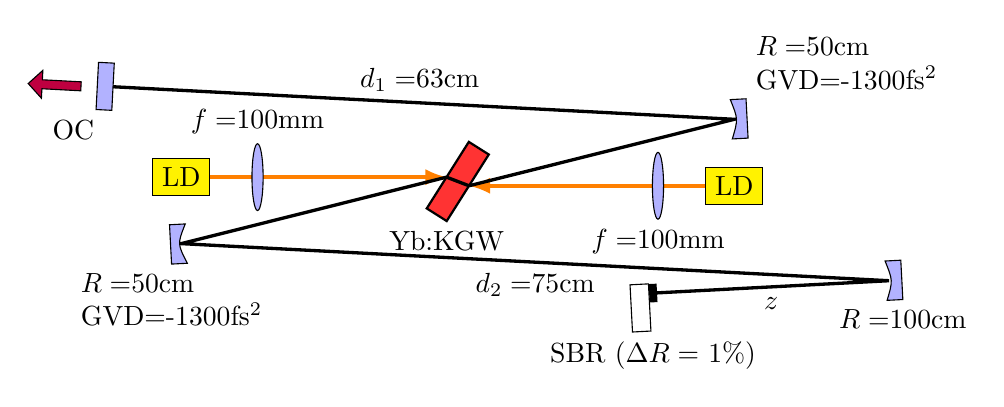
\begin{tikzpicture}
  % laser crystal
  \draw [thick, fill=red!80]
    (0,0) 
    -- ++(-32.3:3mm)
    -- ++(-122.3:10mm)
      coordinate [pos=0.47] (crystal right)
    -- ++(147.7:3mm)
      node [pos=0,below] {Yb:KGW}
    -- ++(57.7:10mm)
      coordinate [pos=0.47] (crystal left)
    -- cycle
  ;
  % beam path in crystal
  \draw [very thick] (crystal left) -- (crystal right);

  % pump lasers
  \node [left=3 of crystal left, fill=yellow, draw] (LD left) {LD};
  \draw [orange, ultra thick, -latex]
    (LD left)
    -- (crystal left)
      coordinate [pos=0.2] (LD lens left)
  ;
  \node [
      draw,
      shape=ellipse,
      inner xsep=0.5mm,
      inner ysep=3mm,
      fill=blue!30,
      label={above:$f=$100mm}
    ]
    at (LD lens left) {};
  \node [right=3 of crystal right, fill=yellow, draw] (LD right) {LD};
  \draw [orange, ultra thick, -latex]
    (LD right)
    -- (crystal right)
      coordinate [pos=0.2] (LD lens right)
  ;
  \node [
      draw,
      shape=ellipse,
      inner xsep=0.5mm,
      inner ysep=3mm,
      fill=blue!30,
      label={below:$f=$100mm}
    ]
    at (LD lens right) {};

  % laser top branch
  \coordinate [above=6mm of LD right] (top turning mirror);
  \draw [very thick]
    (crystal right)
    -- (top turning mirror)
    -- ++(177:8)
      node [pos=0.5,above] {$d_1=$63cm}
      coordinate [pos=1] (OC)
  ;
  \draw [
      fill=blue!30,
    ]
    ($(top turning mirror)+(-0.5mm, 2.5mm)$)
    .. controls ($(top turning mirror)+(3:0.5mm)$)
      .. ++(273:5mm)
    -- ++(3:2mm)
    -- ++(93:5mm)
      node [above right,align=left] {$R=$50cm\\GVD=-1300fs$^2$}
    -- cycle
  ;
  \node [
      draw,
      rectangle,
      inner xsep=1mm,
      inner ysep=3mm,
      fill=blue!30,
      rotate=-3,
      label={below:OC}
    ] 
    at (OC) {}
  ;
  \node [
    draw,
    fill=purple,
    shape=single arrow,
    left=3mm of OC,
    shape border rotate=180,
    single arrow head extend=1.2mm,
    inner xsep=3mm,
    inner ysep=0.5mm,
    rotate=-3
  ] {};

  % laser bottom branch
  \coordinate [below=6mm of LD left] (bottom turning mirror);
  \draw [very thick]
    (crystal left)
    -- (bottom turning mirror)
    -- ++(-3:9)
      node [pos=0.5,below] {$d_2=$75cm}
      coordinate [pos=1] (extension turning mirror)
    -- ++(183:3)
      node [pos=0.5,below] {$z$}
      coordinate [pos=1] (SBR)
  ;
  \draw [
      fill=blue!30,
    ]
    ($(bottom turning mirror)+(0.5mm, 2.5mm)$)
    .. controls ($(bottom turning mirror)+(3:-0.5mm)$)
      .. ++(273:5mm)
    -- ++(3:-2mm)
      node [below,align=left] {$R=$50cm\\GVD=-1300fs$^2$}
    -- ++(93:5mm)
    -- cycle
  ;
  \draw [
      fill=blue!30,
    ]
    ($(extension turning mirror)+(-0.5mm, 2.5mm)$)
    .. controls ($(extension turning mirror)+(3:0.5mm)$)
      .. ++(273:5mm)
    -- ++(3:2mm)
      node [below] {$R=$100cm}
    -- ++(93:5mm)
    -- cycle
  ;

  % SBR
  \node [fill=black,rotate=3,inner xsep=0.5mm] at (SBR) {};
  \node [draw, rotate=3,inner ysep=3mm] at ($(SBR)+(183:1.7mm)+(273:1.8mm)$) {};
  \node [below=5mm of SBR] {SBR ($\Delta R=$ 1\%)};
  
\end{tikzpicture}

\end{document}
